\documentclass[a4paper,11pt]{article}
\usepackage[utf8]{inputenc}
\usepackage[usenames,dvipsnames]{color}
\usepackage{graphicx}
\usepackage[justification=centering,labelfont=bf]{caption}
\usepackage{listings}
\usepackage{csvsimple}
\usepackage{booktabs,mathptmx,siunitx}
\usepackage{minted}
\usepackage{subcaption} 

\definecolor{dkgreen}{rgb}{0,0.6,0}
\definecolor{gray}{rgb}{0.5,0.5,0.5}
\definecolor{mauve}{rgb}{0.58,0,0.82}

\lstset{frame=tb,
  language=C,  
  aboveskip=3mm,
  belowskip=3mm,
  showstringspaces=false,
  columns=flexible,
  basicstyle={\small\ttfamily},
  numbers=none,
  numberstyle=\tiny\color{gray},
  keywordstyle=\color{blue},
  commentstyle=\color{dkgreen},
  stringstyle=\color{mauve},
  breaklines=true,
  breakatwhitespace=true
  tabsize=3
}

\newcommand{\blueline}[1]{\textcolor{blue}{#1}}


\newcommand{\assignatura}{Paral·lelisme}

\newcommand{\titol}{Primera Entrega}

\newcommand{\XXautor}{Sergi Soriano}
\newcommand{\XXXautor}{Mingjian Chen}

\newcommand{\HRule}{\rule{\linewidth}{0.5mm}}

\newcounter{ProblemCounter}
\newcommand{\question}{%
  \setcounter{enumi}{\value{ProblemCounter}}%
  \stepcounter{ProblemCounter}%
}

\newcommand{\answer}[1]{
  {\bf {#1}}
}

\begin{document}

\begin{titlepage}
  \begin{center}
  \textsc{\Large \assignatura}\\[1.5cm]

  \HRule \\[0.4cm]
	{ \huge \bfseries \titol \\[0.4cm] }

  \HRule \\[1.5cm]

  \noindent
	\begin{minipage}{0.4\textwidth}
	\begin{flushleft} \large
	\emph{Autors:}\\
		\large \XXautor \\
		\large \XXXautor
	\end{flushleft}
	\end{minipage}%
	\begin{minipage}{0.4\textwidth}
	\begin{flushright} \large
	\emph{Grup:} 21 
	\end{flushright}
	\end{minipage}


	\vfill

	{\large \today} \\
    {\large \texttt{Facultat d'Informàtica de Barcelona}}
  \end{center}
\end{titlepage}

\section*{Node architecture and memory}
\begin{enumerate}
  \question \item Draw and briefly describe the architecture of the computer in which you are doing this lab session (number of sockets, cores per socket, threads per core, cache hierarchy size and sharing, and amount of main memory).

   \begin{figure}[h!]
    	\begin{center}
  			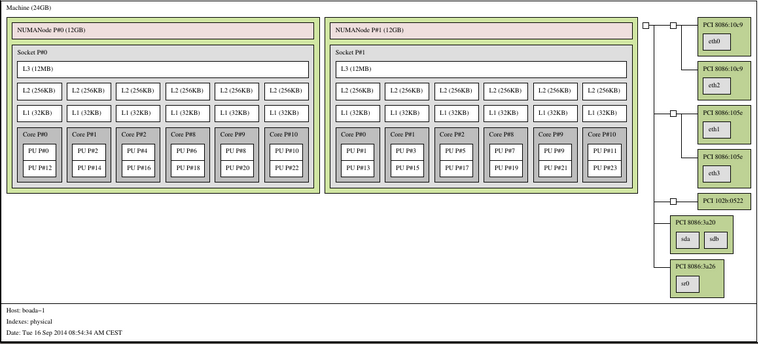
\includegraphics[width=1\textwidth]{architecture_computer.png}
  			\caption{La arquitectura de computador} 
  		\end{center}
  	\end{figure}

  \answer{
    \begin{itemize}
      \item Nombre de sockets: 2
      \item Core per sockets: 6
      \item Thread(s) per core: 2
      \item 3 cache level: L1, L2 i L3
      \begin{itemize}
        \item L1d: 32K
        \item L1i: 32K
        \item L2 : 256K
        \item L3 : 12288K (sharing)
      \end{itemize}
      \item Memoria principal (23.49 GBytes)
    \end{itemize}
  }
\end{enumerate}

\clearpage

  \section*{Timing sequential and parallel executions}
	\begin{enumerate}
	  \question \item Indicate the library header where the structure
	  		struct timeval is declared and which are its fields.

	  \answer{
	    Es definida a \texttt{sys/time.h}.\\
		  Els seus camps són: {\normalfont tv\_sec, tv\_usec}
  		}

	\question \item Plot the execution time when varying the number of threads (strong scalability) 	and problem size (weak scalability) for {\tt pi\_omp.c}. Reason about how the scalability of the program. Tracing sequential and parallel executions.

  \answer{
      Amb el weak scaling podem veure que amb els mateixos threads i augmentant les iteracions, el speed-up que podem conseguir podem dir que és més o menys el mateix.

      En canvi amb el strong scaling, augmentant els threads i una única entrada de iteracions, podem veure que el speed-up que aconseguim a mesura que augmenta les iteracions es més alt, ja que aprofita millor els threads. 
      En el cas del strong scaling veiem que als 7 threads es produeix un overhead.
    }

    \begin{figure}[h!]
      \centering
        \begin{subfigure}[b]{0.65\textwidth}
         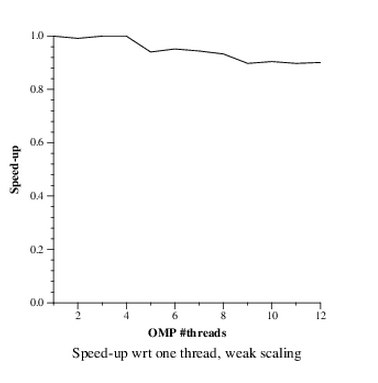
\includegraphics[width=\textwidth]{weak_scalability.png}
          \caption{Weak scalability} 
          \end{subfigure}
    
        \begin{subfigure}[b]{0.65\textwidth}
    			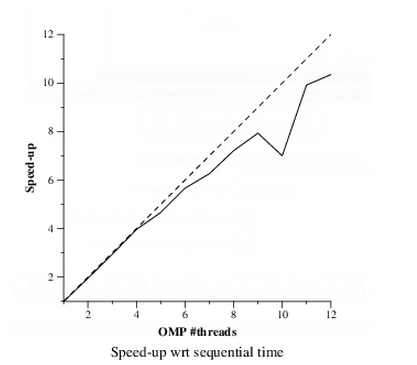
\includegraphics[width=\textwidth]{strong_scalability.png}
    			\caption{Strong scalability}
      \end{subfigure}

     \end{figure}


  	\end{enumerate}
\clearpage

\section*{Tracing sequential and parallel executions}
	\begin{enumerate}
  \question \item From the instrumented version of pi seq.c, and using the appropriate {\bfseries Paraver}      
            configuration file, obtain the value of the parallel fraction for this program when executed with 100.000.000 iterations.

  \answer{
  	El percentatge de la fracció que s’executa en paralel és del 96.63\%.
  }

	\question \item From the instrumented version of {\bfseries pi omp.c}, and using the appropriate Paraver configuration file, show a profile of the \% of time spent in the different OpenMP states {\bfseries ONLY} during the execution of the parallel region (not considering the sequential part before and after) when using 8 threads and for 100.000.000 iterations.

      \begin{figure}[h!]
      \begin{center}
        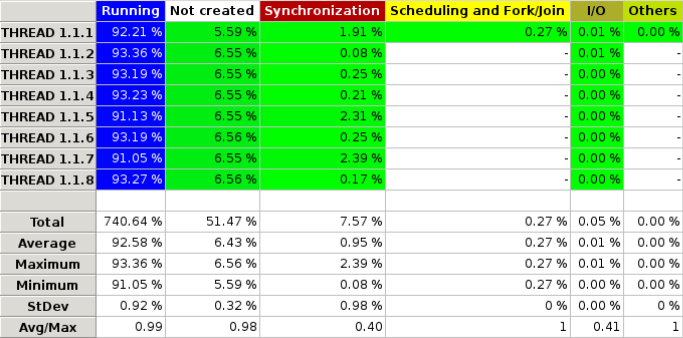
\includegraphics[width=1\textwidth]{pregunta_5.png}
        \caption{\% Time spent in different states} 
      \end{center}
    \end{figure}
    
    \clearpage

    \question \item From the instrumented versions of {\bfseries pi\_seq.c} and {\bfseries pi\_omp.c} (executed with the same number of iterations), and using the appropriate Paraver configuration files, obtain the average number of instructions executed and MIPS per thread during the execution of the parallel region (when using
          8 threads). Are the numbers obtained coherent?

          \begin{figure}[h!]
           \begin{center}
            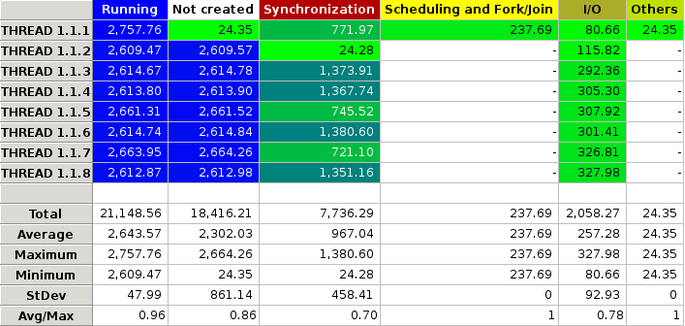
\includegraphics[width=1\textwidth]{pregunta_6_omp.png}
            \caption{pi\_omp} 
            \end{center}
          \end{figure}

            \begin{figure}[h!]
            \begin{center}
              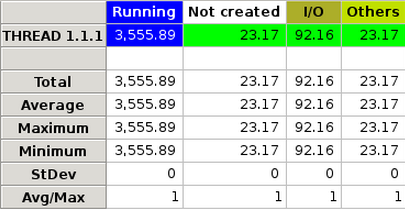
\includegraphics[width=1\textwidth]{pregunta_6_seq.png}
              \caption{pi\_seq} 
            \end{center}
          \end{figure}

          No són coherents. Com bé ens va comentar el professor de laboratori, ve donat per un problema en el contador hardware de la màquina.
          
      \end{enumerate}
  \clearpage

  \section*{Visualizing the task graph and data dependences}
  \begin{enumerate}
    \question \item Include the source code for function {\bfseries dot\_product} in which you show the {\tt Tareador} instrumentation that has been added to study the potential parallelism in the code. This instrumentation has to appropriately define tasks and filter the analysis of variable(s) that cause the dependence(s).

    \begin{lstlisting}
          //dot_product.c
         void dot_product (long N, double A[N], double B[N], double *acc){
            double prod;
            tareador_disable_object(&*acc);
            *acc=0.0;
            int i;
            for (i=0; i<N; i++) {
              tareador_start_task("loop_dot");
              prod = my_func(A[i], B[i]);
              *acc += prod;
              tareador_end_task("loop_dot");
            }
            tareador_enable_object(&*acc);
          }
    \end{lstlisting}

    \clearpage

    \question \item Capture the task dependence graph and execution timeline (for 8 processors) for 
                that task decomposition.
      \begin{figure}[h!]
        \begin{center}
        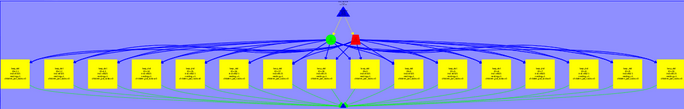
\includegraphics[width=1.2\textwidth]{pregunta_8_1.png}
        \caption{Figure task dependence grahp \texttt{dot\_product.c}}
        \end{center}
      \end{figure}

      \begin{figure}[h!]
        \begin{center}
        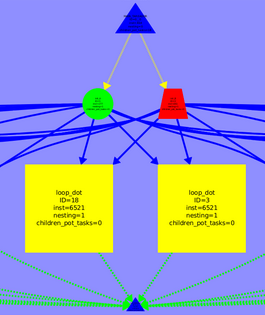
\includegraphics[width=0.7\textwidth]{pregunta_8_2.png}
        \caption{Figure task dependence grahp ampliado \texttt{dot\_product.c}}
        \end{center}
      \end{figure}

      \begin{figure}[h!]
        \begin{center}
        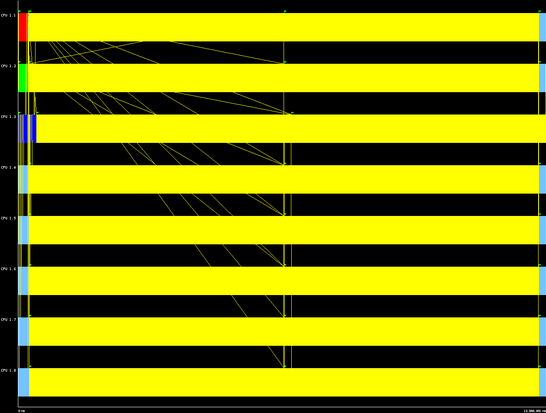
\includegraphics[width=1\textwidth]{pregunta_8_3.png}
        \caption{Figure timeline \texttt{dot\_product.c}}
        \end{center}
      \end{figure}
  \end{enumerate}
\clearpage

\section*{Analysis of task decomposition}
    \begin{enumerate}

      \question \item Complete the following table for the initial and different versions generated for {\tt 3dfft\_seq.c}.
      \begin{center}
        \begin{tabular}{| c || c | c | c |}
          \hline
              {\bf Version} & $T_1$ & $T_{\infty}$ & {\bf Parallelism} \\
              \hline
              \hline
              sqe & 593762 & 593747 & 1.000 \\
              \hline
              v1 & 593762 &  593747 &  1.000 \\
              \hline
              v2 & 593762 & 315188 & 1.884 \\
              \hline
              v3 & 593762 & 108336 & 5.481 \\
              \hline
              v4 & 593762 & 59412 & 9.994 \\
              \hline
        \end{tabular}
      \end{center}

      \question \item With the results from the parallel simulation with 2, 4, 8, 16 and 32 processors, draw the execution time and speedup plots for version {\tt v4} with respect to the sequential execution (that you can
        estimate from the simulation of the initial task decomposition that we provided in {\tt 3dfft\_seq.c},
        using just 1 processor).

        \begin{center}
          \begin{tabular}{| c || c | c |}
            \hline
                {\bf Processors } & {\bf Time (ns)} & {\bf Speed-up} \\
                \hline
                \hline
                1 & 593,762,001 & 1 \\
                \hline
                2 & 297,297,001 & 1.997 \\
                \hline
                4 & 156,077,001 & 3.804 \\
                \hline
                8 & 86,558,001 & 6.860 \\
                \hline
                16 & 59,412,001 & 9.994 \\
                \hline
                32 & 59,412,001 & 9.994 \\
                \hline
          \end{tabular}
        \end{center}

        \clearpage

        \begin{figure}[!ht]
          \begin{center}
          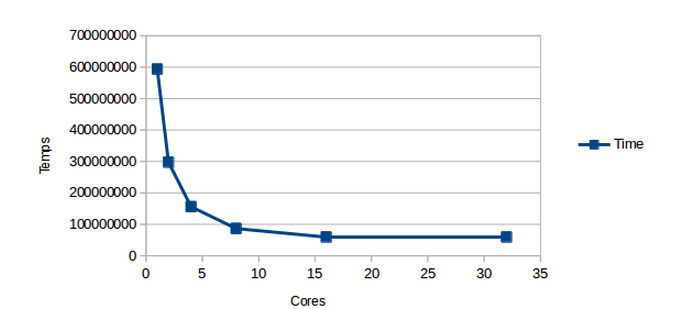
\includegraphics[width=1\textwidth]{temps_cores.png}
          \caption{Figure execution timeline en funció del nombre de cores}
          \end{center}
        \end{figure}

        \begin{figure}[!ht]
          \begin{center}
            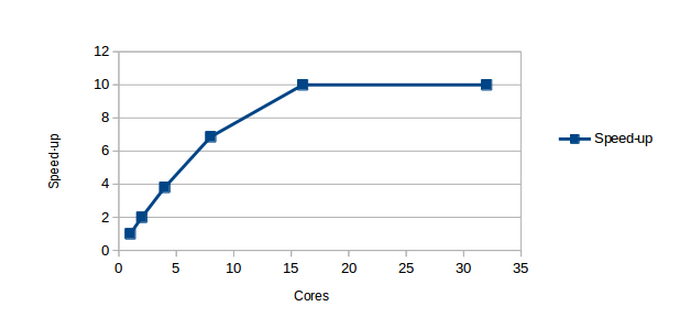
\includegraphics[width=1\textwidth]{speedup_cores.png}
          \caption{Figure Speed-up en funció del nombre de cores}
          \end{center}
        \end{figure}

  \end{enumerate}

\end{document}

